\title{CS 181 Practical Writeup}
\author{
        Kevin C. Ma, Robert Chen, Richard Zou
}
\date{\today}

\documentclass{article}
\usepackage{amssymb} %general math
\usepackage{mathtools} %text in formulae and more advanced stuff
\usepackage{verbatim} %multiline comments with \begin{comment}
\usepackage{geometry}
\geometry{%
  letterpaper,
  lmargin=2cm,
  rmargin=2cm,
  tmargin=2cm,
  bmargin=2cm,
  footskip=12pt,
  headheight=12pt}

\usepackage{fancyhdr}
\pagestyle{fancy}

%\cfoot{Page \thepage\ of \totalpages}


% Creates the square box used to end a solution.
\def\squarebox#1{\hbox to #1{\hfill\vbox to #1{\vfill}}}
\def\qed{\hspace*{\fill}
        \vbox{\hrule\hbox{\vrule\squarebox{.667em}\vrule}\hrule}}
\newenvironment{solution}{\begin{trivlist}\item[]{\bf Solution}}
                      {\qed \end{trivlist}}
\newcommand{\set}[1] { \{#1\} }
\newcommand{\whitespace}{ \vspace{\baselineskip} }
\newcommand{\inner}[1]{\left< #1\right>}
\newcommand{\norm}[1]{\| #1 \|}
\newcommand{\ans}[1]{\Aboxed{#1}}

\usepackage{mathtools}
\DeclarePairedDelimiter{\ceil}{\lceil}{\rceil}
\DeclarePairedDelimiter{\floor}{\lfloor}{\rfloor}

\begin{document}
\maketitle

\section{Introduction}

Our approach to predicting the HOMO-LUMO gap employed linear regression methods, random forests, and neural networks. We found that a random forest regressor performed moderately well relative to the class and that there were opportunities for further improvement of the basic model by increasing the number of predictors from RDkit's fingerprinting feature [5]. In all of these models, due to time and computational power constraints, we trained on data from the first 50,000 molecules and used subsequent sets of 50,000 molecules as validation sets.

\section{Basic Regression Techniques}

\subsection{Initial Runs}

We first utilized the benchmark techniques: simple linear regression and ridge regression with the default coefficient weight for the penalty term ($\alpha$) of 0.5. When running these on our 50,000 molecule sample sets, we obtained RMSE values of .29820072 and .29818009, respectively. We also ran these regression techniques in the Kaggle competition, and based on those results, we concluded that the 50,000 molecule sample yielded accuracy scores sufficiently similar to the actual test data, and differences in performance of separate techniques was especially sufficiently reflective of differences in test data performance between those techniques.

\subsection{Ridge Regression Cross Validation}

We used a standard cross validation approach, as has been discussed in section, in order to determine an optimal alpha value for ridge regression. To do this, we utilized the scikit-learn RidgeCV function [6]. This yielded an alpha value of 1.175; however, the performance with this alpha value was relatively negligible in comparison to the default ridge regression, reflecting inherent complexity in the data that could not be modeled using the ridge regression technique.

\subsection{Lasso Regression and Elastic Net Regularization}

Similar issues were encountered when trying lasso regression. In comparison to ridge regression, lasso regression tends to deselects some features by driving their weight in the regression to 0 as the alpha parameter is increased. We used the Elastic Net method, which allows for a mixture between ridge and lasso by minimizing the same least squares expression as ridge and lasso, but with penalty term of $\frac{\alpha (1-\rho )}{2} \sum_1^J |w_j|^2 + \frac{\alpha \rho }{2} \sum_1^J |w_j|$, for $0 \leq \rho \leq 1$.

We found that the model, under cross validation of the alpha and rho parameters using ElasticNetCV, chose a rho of 0, which corresponds to completing favoring ridge regression. As expected, the optimal alpha value was 1.175, the same as under testing with RidgeCV.

\section{Random Forest Regression}

\subsection{Background}

Next we consider the random forest regression method, which is an ensemble algorithm that is quite efficient yet often quite accurate for large data sets [7]. It employs a decision tree classification idea and averages performance over numerous decision trees. Each decision tree uses a random sample of the training data (drawn with replacement). To complete the classification within each tree, one completes a series of binary splits which divides the data subsequently into groups. For each split, a random sample of features is compared. For each feature, one optimizes the residual sum of squares; that is, one picks the value that creates two groups (above [A] and below [B] the value) such that the expression $\sum_A (y_A - \mu _A)^2 + \sum_B (y_B - \mu _B)^2$ is minimized, where $\mu _A, \mu _B$ are the respective means of the two groups. Then, take the minimum of this number over all the features to use as the split. At the end, the value assigned to each leaf node group is the average of the target values for the members of that group. Given the regressor, categorizing test data just amounts to following each tree down through the splits, and then averaging the values obtained from the resulting leaf node group of each decision tree. [8] [9]

One parameter to set through testing is the number of features that are randomly chosen to be compared at each split. Also, the greater the depth of the trees utilized before stopping the procedure, the smaller the bias; however, this requires a much higher number of trees (another parameter) in order to maintain relatively low variance. Higher numbers of trees will generate more accurate predictions, but with diminishing returns.


\subsection{Model Selection}

Upon investigating different max number of features to select from at each split, we found there to be very small difference between using the square root of the number of features, the base-2 log of the number of features, and our scikit-learn function RandomForestRegressor's default setting of using all features. We ultimately worked with the square root, which gave the (marginally) best RMSE error in our tests. We changed the default setting of using 10 decision trees in the random forest to using 300 trees, after our tests revealed diminishing returns to increasing the number of trees at around 300, but somewhat significant improvements up until that point. See graph in Figure 1 (on the last page of the document).

\subsection{Error Analysis and Post-Prediction Adjustments}

Using 50,000 molecules as the training set and 50,000 molecules as the test set with the random forest model yielded a RMSE of about .276. To analyze this error, we plotted Actual Gap Value vs. Error (Actual - Predicted Value) [Figure 2] and Predicted Gap Value vs. Error (Actual - Predicted Value) [Figure 3]. From Figure 2, we see that our random forest is consistently underestimating high gap values and overestimating low gap values; that is, the predictions are not extreme enough, mainly instead staying around the mean. Such underfitting is also reflected in how RMSE on train and test data is about the same and in how taking the average of predictions for random forests and ridge regression, a mixture as in the Netflix Prize approaches, was unsuccessful (the two models underfit in the same direction).

However, we don't know the actual values when doing an actual prediction. Unfortunately, as shown in Figure 3, we cannot make out as much of a pattern when considering only observed prediction values. We can still artificially correct for this small amount of error, however, by fitting a polynomial curve to the Figure 3 data. Then, given actual test data, we can make our prediction using random forest and then add on the correction number as given by the polynomial for each prediction value to reduce the RMSE. This depends on using the same training data to generate the regressor for the validation data (which generates the polynomial) and the actual test data.

With 50,000 molecule training and validation sets, we fit polynomials (Degree 2, 3, and 5 shown in Figures 4-6). Based on tail behavior and overfitting to outliers in the data, we used the cubic $-0.09511856x^3+0.53458563x^2-0.98841412x+0.60673527$ to compute corrections. Testing on a third set of 50,000 molecules yielded sizably better RMSE scores than without the adjustment.

\subsection{Training Set Size's Impact on Error}

To make our best predictions on the actual test data, we needed to use a random forest trained on a much larger amount of the given 824,230 molecules. With a new training set, we also need a new validation set to determine a polynomial for the adjustment. Thus we used 700,000 molecules to train the random forest and the remaining 124,230 molecules to determine a polynomial. Unfortunately, we did not previously anticipate that this time, the polynomial generated negligible corrections for predictions, and thus RMSE was only very slightly better (about .00001) than for just the random forest regressor on its own. [Figure 7] In fact, a better RMSE could be obtained by simply using all 824,230 molecules as training data; the benefit of more training data eclipsed that of the polynomial correction. We thus conclude that the polynomial correction previously worked because the training sample size was too small to fully capture the power of random forests; with enough training data, the random forest's predictions are unbiased. After that, there is simply an inherent limit to the ability for random forests to make good predictions on this data.



\section{Artificial Neural Network Regression}

\subsection{Background}

Artificial neural networks (ANN) are a set of biologically inspired algorithms
for machine learning.  There is a neural network net, composed of a set of input
 nodes in the first layer, hidden nodes (in zero or more hidden layers), and output
  notes in the last layer. All the nodes in one layer are connected to all the nodes 
  in the next layer.  A neural network takes in a vector as input (each node takes an 
  element of the vector).  Then, the nodes “fire” based on an activation function: 
  for a non-linear activation function such as the sigmoid or hyperbolic tangent, 
  each node will send a signal to its connections based on how large or small the 
  input to them was.  Each node in the second layer collects all of the inputs from 
  the previous layer and weighs them linearly by weights on the connections, and then
   fires again according to the activation function to the third layer.  Finally, 
   the output layer will have the output of the neural network; for a regression 
   problem like this, there is one output node which will output a value, a 
   weighted linear combination of the nodes that fired in the previous layer. [1]

Most of the work done in artificial neural networks research
 involves the creation of
 learning algorithms to optimize the weights between nodes.  [3]
 

\subsection{Setting up an ANN}

We decided to use the Torch7 machine learning library to create and 
train an artificial neural network [2].  Installing and
 setting up dependencies took a rather long time.  Ultimately, we were
  able to run Torch7 on Ubuntu 14.04 LTS on a 4.0GHz Intel i7 processor
   and a Nvidia GeForce GTX 750 Ti graphics card with GPU acceleration. 
    Training a neural network on the GPU rather than the CPU resulted in
     five to twenty time speedups, well worth the initial time investment
      in setting up the dependencies.


\subsection{Training algorithm}
The training algorithm is where the optimization of the neural network
 occurred and the ``heart'' of the machine learning.  We implemented 
 a simple backpropagation algorithm that involved gradient descent.  In 
 preparation for this, we used a tanh activation function for all of the
  nodes (to use gradient descent, the activation function has to be differentiable). 
   The backpropagation algorithm sends error signals backwards through the neural
    network to update the weights to minimize the error loss function, which we
     defined as the mean squared error.  Minimizing the mean squared error is
      the same as minimizing our root mean squared error. [4]

\subsection{Desiging our ANN}
Initially, we designed the neural network with 256 input nodes
 (one for each element in the feature vector), and 1 output node
  (for the output).  We trained it for 100 iterations on the first 
  10,000 rows of the data, and then tested its performance on the 
  second 10,000 rows of the data.  This resulted in a RMSE error of
   around 0.2994.  Without a hidden layer, the neural network almost
    does the same thing as linear regression: it takes the feature
     vector, performs some linear operation to it, then performs a 
     nonlinear operation (tanh) and then returns an answer.  To do better
      learning, we would have to add a hidden layer to the ANN.

Now, the problem at hand was finding a good structure for the neural network. 
 We experimented with 
32, 64, 128, 256, 512, and 1024 hidden layers, using 3-fold cross
validation for a total set of 30,000 random rows (same rows for each test,
this took us a few hours).
Below is a table of the RMSE after training for 200 iterations and
a learning rate of 0.01:

\begin{tabular}{ c | c }
  Nodes in hidden layer & Average RMSE of the model  \\
  32 & 0.29403  \\
  64 & 0.29489  \\
  128 & 0.29319 \\
  256 & 0.29314 \\
  512 & 0.29296 \\
  1024 & 0.29342 \\
\end{tabular}

Unfortunately, we were unable to differentiate between 
the performance of different numbers of hidden nodes because 
of how close the RMSE values are to each other.  In general,
there should be a balance between too few nodes (underfitting)
and too many nodes (overfitting), but we did not notice
either underfitting or overfitting.  However, in an experiment
on a smaller set of the data, a 3-fold cross-validation on a total of
300 randomly chosen elements, we found a lot of overfitting as the number of
nodes increased.

To better understand how the training algorithm performed,
we can look at a graph of the internal root mean squared error
of the model during training at each iteration of the stochastic
gradient descent algorithm.  In the end, we worked mostly with
the neural network with 128 hidden nodes for speed purposes.

% 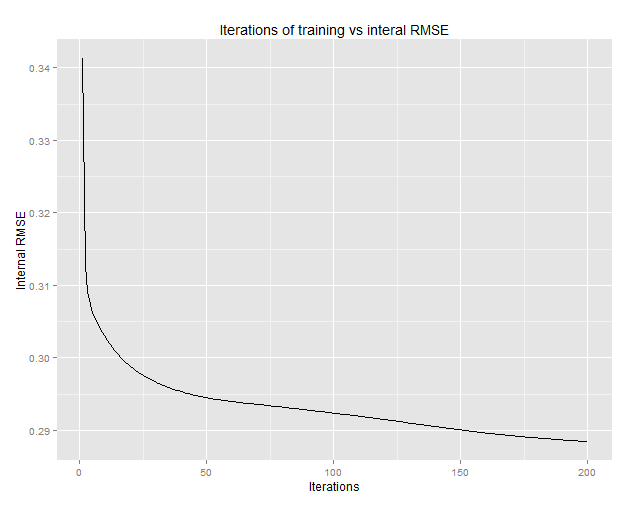
\includegraphics[scale=0.5]{run128.png}

The main bottleneck that we faced was time: at 200 iterations, it seems
as if the curve, the internal RMSE, levels off and does not
decrease very much.  After around 600 iterations (we did not
record the internal data for this, only the end result),
the internal RMSE was 0.27711, showing diminishing marginal
returns.  The interal RMSE is a lower
bound on the performance of any model on new data, so we chose
not to proceed with the neural network model in the interest
of time and efficiency.

\subsection{Results and conclusion for ANNs}
With our neural network structure, we were unable to see any large 
improvements over the simple ridge linear regression method.  
We suspect
 that this may have been due to the quality of the data 
 - our neural networks seemed to 
 have a difficult time predicting values even with a good training
 algorithm.  Perhaps the features of the smiles string do not correlate
 very much with the energy gap.  If we had more time, we would have
 went into RDKit to extract more relevant features that may pertain more
 to the energy gap and train the neural network on these larger
 vectors.  Determining which elements of the features vector
 to keep and which not to keep would also help in a neural networks approach.

\section{References and Citations}


\begin{description}
  \item{[1]} http://www.willamette.edu/~gorr/classes/cs449/intro.html
  \item{[2]} http://torch.ch/
  \item{[3]} http://neuralnetworksanddeeplearning.com/chap2.html
  \item{[4]} http://torch.cogbits.com/wiki/doku.php
  \item{[5]} http://www.rdkit.org/docs/GettingStartedInPython.html
  \item{[6]} http://scikit-learn.org/stable/modules/generated/sklearn.linear\_model.RidgeCV.html
  \item{[7]} http://scikit-learn.org/stable/modules/ensemble.html
   \item{[8]} http://www.bios.unc.edu/~dzeng/BIOS740/randomforest.pdf
    \item{[9]} http://www.math.usu.edu/adele/randomforests/uofu2013.pdf
\end{description}

\end{document}
